\documentclass[12pt]{galois-whitepaper}
\usepackage{listings}
\usepackage{float}
\usepackage{xspace}
\usepackage{color}
\usepackage{tikz}
\usepackage{url}
\usepackage{amsmath}
\usepackage{amscd}
\usepackage{verbatim}
\usepackage{fancyvrb}
\let\verbatiminput=\verbatimtabinput
\VerbatimFootnotes
\DefineVerbatimEnvironment{code}{Verbatim}{}
\DefineVerbatimEnvironment{pseudoCode}{Verbatim}{}
\hyphenation{Saw-Script}
\newcommand{\sawScript}{{\sc SawScript}\xspace}
\renewcommand{\textfraction}{0.05}
\renewcommand{\topfraction}{0.95}
\renewcommand{\bottomfraction}{0.95}
\renewcommand{\floatpagefraction}{0.35}
\setcounter{totalnumber}{5}
\definecolor{MyGray}{rgb}{0.9,0.9,0.9}
\makeatletter\newenvironment{graybox}{%
   \begin{lrbox}{\@tempboxa}\begin{minipage}{\columnwidth}}{\end{minipage}\end{lrbox}%
   \colorbox{MyGray}{\usebox{\@tempboxa}}
}\makeatother

\setlength{\parskip}{0.6em}
\setlength{\abovecaptionskip}{0.5em}

\lstset{
         basicstyle=\footnotesize\ttfamily, % Standardschrift
         %numbers=left,               % Ort der Zeilennummern
         numberstyle=\tiny,          % Stil der Zeilennummern
         %stepnumber=2,               % Abstand zwischen den Zeilennummern
         numbersep=5pt,              % Abstand der Nummern zum Text
         tabsize=2,                  % Groesse von Tabs
         extendedchars=true,         %
         breaklines=true,            % Zeilen werden Umgebrochen
         keywordstyle=\color{red},
                frame=lrtb,         % left, right, top, bottom frames.
 %        keywordstyle=[1]\textbf,    % Stil der Keywords
 %        keywordstyle=[2]\textbf,    %
 %        keywordstyle=[3]\textbf,    %
 %        keywordstyle=[4]\textbf,   \sqrt{\sqrt{}} %
         stringstyle=\color{white}\ttfamily, % Farbe der String
         showspaces=false,           % Leerzeichen anzeigen ?
         showtabs=false,             % Tabs anzeigen ?
         xleftmargin=10pt, % was 17
         xrightmargin=5pt,
         framexleftmargin=5pt, % was 17
         framexrightmargin=-1pt, % was 5pt
         framexbottommargin=4pt,
         %backgroundcolor=\color{lightgray},
         showstringspaces=false      % Leerzeichen in Strings anzeigen ?
}

\author{Levent Erk\"{o}k $\;\;\;\;\;$ Joe Hendrix\\
\texttt{\{levent.erkok,jhendrix\}@galois.com}}
\title{\sawScript}
\date{February 2011}
\begin{document}
\maketitle

\vspace*{2cm}
\begin{abstract}
We introduce the \sawScript language, aiming to provide
a programmable interface to Galois's Java Verifier and Cryptol based
formal verification technologies. We use various simple Java programs as examples, inspired
the domain of elliptic-curve cryptography. Our proofs either directly take place within the
\sawScript specification language, or use \sawScript to equivalence check Java functions against
their Cryptol counterparts.
\end{abstract}

\newpage
\tableofcontents
\newpage

\section{Introduction}
\sawScript is a proof scripting language and its associated proof engine, aimed at simplifying the use of Galois's Java Verifier and Cryptol~\cite{Cryptol} based
verification technologies. \sawScript allows concise descriptions of proof steps, freeing the users from the details
of how the proofs are actually constructed and run.

\paragraph{NB} While this initial version of \sawScript closely reflects our experiences with proofs about Java and Cryptol
programs, we consider it a general tool for describing proofs for programs written in arbitrary languages.
Therefore, the surface
syntax of \sawScript is likely to evolve as we add capabilities on both the proof construction and specification
aspects, and as we focus on supporting other languages, such as LLVM or C.

\section{Basics}
In this section we will consider a couple of very simple Java programs and see how we can specify and prove them correct
using \sawScript.

\subsection{Checking that an array is properly reset}
Consider the following Java method:
\begin{Verbatim}
  static private boolean is_zero(int[] x) {
     for (int i = 0; i != x.length; ++i) {
       if (x[i] != 0) return false;
     }
     return true;
   }
\end{Verbatim}
The function {\tt is\_zero} takes a reference to an arbitrary sized integer array, and returns {\tt true} if all the elements
are set to {\tt 0}, i.e., if the array is properly reset. In our first example, we will see how we can write a
specification for this function, and prove that it is correct using \sawScript.

\paragraph{NB} We should emphasize that all Java proofs in \sawScript are done over the corresponding JVM bytecode. While Java programmers
typically do not think in terms of JVM during day-to-day programming, there are subtle details that do come up when
we try to prove properties of Java programs in this way. We will try to point out these differences explicitly as necessary.

Given the {\tt is\_zero} Java method above, here is how we would express the proof that it does indeed check that
its argument is properly set to all {\tt 0}s in \sawScript:

\begin{code}[numbers=left]
  method com.galois.ecc.P384ECC64.is_zero {
    var args[0] :: int[12];
    return join(valueOf(args[0])) == 0:[384];
    verify abc;
  };
\end{code}
Let us walk through this proof script in detail to explain the basic concepts behind \sawScript:

\paragraph{Lines 1, 2} Java has {\tt boolean}s as a built-in type with only possible values {\tt true} and {\tt false}
as inhabitants. JVM, however,
represents booleans simply as 32-bit integers, with values $1$ and $0$, respectively~\cite[Section 3.3.4]{Lindholm:1999:JVM:553607}.
Therefore, the booleans at the Java level have to be treated properly as integers when we encode proofs over the corresponding JVM
representation.  Since truth values come up quite often, we simply create two constants with the respective values. 

Following the Cryptol notation, word types are written {\tt [n]}, where {\tt n}
is the bit-size. Note that we do not distinguish between signed and unsigned words at this level: We are merely stating that there are 32
bits available: How those bits are interpreted is up to the individual operations that act on these values. You will also notice that
\sawScript requires annotations on all constants, i.e., the type specification {\tt [32]} is mandatory on the constants $1$ and $0$.

\paragraph{Line 4} This is where the property specification starts for the {\tt is\_zero} method. We tag it with its class name,
which happens to be {\tt com.galois.ecc.P384ECC64} in this case. Note that \sawScript will follow the Java inheritance hierarchy
to find the method {\tt is\_zero} in this class: It can either be directly defined in that class, or it can be defined in any one
of its superclasses: \sawScript will properly locate it, and will complain if it cannot.

\paragraph{Tip} To be able to locate java classes, you will need to tell \sawScript the class and {\tt jar} paths as installed
on your system. See the {\tt -c} and {\tt -j} options of \sawScript for details. (You can issue {\tt sawScript --help} to see
all available options.)

\paragraph{Line 5} The first thing we do in a method specification is to provide the type information for the arguments to the method.
The {\tt var} declaration states that the first argument to the method, i.e., {\tt arg[0]}, is an array of length 12, containing
Java {\tt int}s. We write this type in \sawScript like this: {\tt int[12]}.

\paragraph{NB} The attentive reader would have no doubt wondered how we came up with the number 12 for the length of our array. After
all, the Java program we have given works for arrays of arbitrary sizes, not just 12. (Using Cryptol terminology, we would say that
the Java method {\tt is\_zero} is size polymorphic.) Ideally, we would like to be able to say that the property holds for arbitrary
arrays. Unfortunately, \sawScript currently only allows for monomorphic specifications: We cannot write polymorphic properties. This
is not a mere limitation of the current implementation of \sawScript: As we have demonstrated before in the context of Cryptol, one cannot
expect to be able to automatically prove arbitrary polymorphic properties of bit-precise programs~\cite{erkok-matthews-cryptolEqChecking-09}.

In \sawScript, we
aim for push-button automated verification, and hence we focus our attention on monomorphic properties only. Therefore, we have to give
a fixed constant size for the array, and in this case we choose that number to be 12. (While it's unlikely that this monomorphism restriction
will ever be completely removed from \sawScript, future versions might relax the requirements, and allow for some parametric proofs to be encoded directly.)

\paragraph{Lines 6-9} At this point, we are ready to describe the desired behavior of the {\tt is\_zero} method directly in \sawScript. This is the goal
of the {\tt returns} statement. The expression on the right hand-side is a direct encoding of how we would expect this method to work: If the argument
has all 0 elements, then it should return {\tt true}, otherwise it should return {\tt false}. Keeping in mind how JVM represents Java booleans
the {\tt then} and {\tt else} branches (lines 8 and 9) merely encode that specification.

To understand how the specification is given, let us consider the test-expression (line 7) in more detail:

\begin{verbatim}
        join(valueOf(args[0])) == 0:[384]
\end{verbatim}

Here are the constituents:
\begin{itemize}
\item {\tt args[0]}: This is the first argument to the {\tt is\_zero} method, that we declared to have type {\tt int[12]} on line 5. Most importantly,
this is a Java value, and not a \sawScript value.
\item {\tt valueOf}: This function lifts values from the Java world into \sawScript. 
Whenever we refer to a Java value (such as {\tt args[0]}), we have to
explicitly bring it to the \sawScript level using {\tt valueOf}. This two-level type-system is crucial in keeping the two worlds separate: The object level at which
Java operates, and the proof level at which \sawScript works. The {\tt valueOf} call basically tells \sawScript to take the Java value and bring it to the
level where we write the specifications.
\item {\tt join}: The function {\tt join} is a primitive in \sawScript, similar to Cryptol's {\tt join}. It takes a sequence of words and joins them
together to make one big word out of them. In this case, its argument is a 12 element array containing 32-bit values, and hence it returns a $12\times32 = 384$
bit word.
\item {\tt 0:[384]}: This is the \sawScript constant 0 at 384 bits.
\end{itemize}

In summary, the {\tt returns} statement on lines 6-9 is telling \sawScript that when the method {\tt is\_zero} completes execution, it will return
{\tt javaTrue} (i.e., 1:[32]) if all the elements of the input array are equal to 0, and {\tt javaFalse} (i.e., 0:[32]) otherwise. This is how we capture
the operation of the Java method as a functional \sawScript specification.

\paragraph{Line 10} Finally, the user is giving a hint to \sawScript to use the the {\tt abc} tool to verify this specification, essentially showing
correctness using first bit-blasting and then discharging the associated verification conditions
using Mishchenko's  ABC tool~\cite{ABC}. The other possible values are {\tt rewriter} and {\tt auto}.
The {\tt rewriter} tactic tries the internal rewriting engine to show correctness, while the latter first rewrites and tries {\tt abc} on the remaining subgoals, 
i.e., it's a hybrid of {\tt abc} and {\tt rewriter}. Users can also specify
\begin{Verbatim}
  verifyUsing: skip;
\end{Verbatim}
which means that \sawScript should not attempt to prove the specification at all.

\paragraph{NB} In this particular example, the proof is
specified directly within \sawScript's specification language: We do not perform equivalence checking, but rather
state and prove the property directly within \sawScript. Later on, we will also see how to use \sawScript to equivalence check Java programs
against Cryptol reference implementations.

If you were to try this example using \sawScript, you will see that the proof completes instantaneously with success. If the specification was in error, then
\sawScript will print a counter example if the {\tt abc} tactic is used, or the final verification condition that it failed to discharge.
(See Section~\ref{sec:proofexec} for details.)

\subsection{Resetting an array}
The {\tt is\_zero} method of the previous section introduced the basic concepts behind
\sawScript. One important thing to note about {\tt is\_zero} is that it is a function without
any side effects: It does not modify its arguments.
The goal of this
section is to illustrate how we can prove properties of Java programs that do modify their arguments.
We will do so by studying the corresponding Java procedure that sets the elements
of its argument array to all {\tt 0}s:

\begin{Verbatim}
  static void set_zero(int[] x) {
    for (int i = 0; i != x.length; ++i)
       x[i] = 0;
  }
\end{Verbatim}

Unlike {\tt is\_zero}, {\tt set\_zero} does not return any values, but rather simply wipes out the elements of the given array. We would
like to state that it indeed zeros out the given array as a property, and prove it correct using \sawScript. Here is the corresponding functional specification:
\begin{code}[numbers=left]
  method com.galois.ecc.P384ECC64.set_zero {
    var args[0] :: int[12];
    ensure valueOf(args[0]) := split(0:[384]) : [12][32];
    verify abc;
  };
\end{code}
What is new in this specification is the use of the {\tt ensures} clause (line 3). What {\tt ensures} allows us is to state precisely
what observable modifications the Java method will have performed
after it {\em completes} its execution. In this case, we are stating that {\tt args[0]} must essentially be
equivalent to the 384-bit value {\tt 0} split into an array of length 12, containing all 0 elements.

\paragraph{NB} Similar to the specification for {\tt is\_zero}, the above property is stated for arrays of length
12, even though the corresponding Java method can accept
arrays of arbitrary size. Also, you will find that \sawScript requires type annotations for uses of the {\tt split} function, similar to the
mandatory annotations on constants.

A given specification may contain both a {\tt returns} clause and multiple {\tt ensures} clauses, as necessary. If you were to try the
above example using {\tt sawScript}, you will again see that the proof completes instantaneously.

\subsection{Basic execution of a \sawScript proof}\label{sec:proofexec}

Before moving on to bigger examples, and in particular to equivalence checking
between Java and Cryptol, let us take a moment to summarize how a basic
\sawScript proof proceeds. 
When \sawScript first encounters the specification, it first typechecks it
to ensure that the Java, Cryptol, and \sawScript types are compatible and
used in a consistent way.  This initial typechecking can catch many early
specification bugs, resulting in huge time savings from a development/evaluation perspective.

Unless the directive ``{\tt verifyUsing:} {\tt skip}'' is given by the user, \sawScript will perform the following actions
on each method specification:

\begin{enumerate}

\item Search the current class search path to locate the correct Java class.

\item Find the corresponding method body to be verified, by looking in the
        Java class thus located, and its superclasses.

\item Create an initial simulator state, with symbolic input values derived
        using the type information from the {\tt var} declarations, and
        constants from the {\tt const} declarations.  
        \label{enum:simulator}

\item Run the method symbolically on these inputs, using the symbolic
        simulation capabilities supported by the Java Symbolic Simulator
        ({\tt{}jss}),

\item Compare the final JVM state returned by the symbolic simulator against
        the values specified in the method specification {\tt returns} and
        {\tt ensures} statements.  The main steps in this comparison are to:
        
 \begin{itemize}

   \item Identify any new memory that was allocated for classes not in the current
           specification, or modified fields that were not specifically
           mentioned in the specification.  If either new memory is allocated, or unexpected
           modifications are found, fail immediately with an appropriate message.

   \item Iterate through the defined field values, arrays, and the {\tt return} statement.
           For each one, generate a \emph{equivalence condition} $v_i = s_i$ asserting
           that the value $v_i$ from the symbolic simulator equals the relevant
           specification value $s_i$ obtained from the \emph{ensures} clause.
           If no \emph{ensures} clause is defined for the value, then
           the specification value $s_i$ is the value in the initial state, i.e., it must
           not have been modified by the method.

 \end{itemize}

 \item Combine the assumptions $a_1, \dots, a_n$ defined in the specification
         with the equivalence conditions from the previous step to generate a single
         verification condition:
       \[ a_1 \wedge \dots \wedge a_n \implies
         v_1 = s_1 \wedge \dots \wedge v_{n'} = s_{n'}.\]

 \item Use the user specified verification tactic to attempt to reduce the verification
         condition to {\tt True} in all cases.  If the tactic fails to discharge the
         verification goal, we report the failure to the user along with any
         relevant information to help understand the failure.
         
 \item Once a specification has been processed, the symbolic simulator will
         use the specification instead of the Java bytecode in symbolically
         simulating later methods.  This capability not only accelerates symbolic
         simulator performance, but is essential for the compositional
         verification of methods that produce proof terms too large for automated
         technologies (SAT or otherwise) to handle.
           
\end{enumerate}

SAWScript currently supports two main verification tactics: (1) using rewriting
to simplify or solve a verification condition; (2) applying bitblasting to
generate an And-Inverter Graph (AIG) from the verification problem, and sending
it to the ABC equivalence checker for verification.  These verification
tactics can either be used by themselves, or combined into a single \emph{auto}
tactic which first applies the rewriter to simplify the problem, and then
generates an AIG for the simplified result.

The two verification tactics are useful in different situations.  Using the
\emph{abc} tactic is much more automatic, but \emph{abc} may fail to terminate
on a verification problem in a reasonable amount of time, 
without providing any insight into why.  Using the
\emph{rewriting} tactic is a more labor intensive affair, and requires the
\sawScript author to invest effort in coming up with a suitable set of rewrite rules
to solve the verification problem. However, when the right rules are used, the
rewriting based proofs can go much faster, as we shall see later in Section~\ref{sec:rules}.

The verification tactic also has an impact on what information is returned
to the user when verification fails:
\begin{itemize}

  \item If the {\tt abc} or {\tt auto} tactics are used and {\tt abc} is able
          to generate a counterexample, then \sawScript will display the
          counterexample to the user with a detailed description of what Java
          input values triggered it, and how the expected and
          actual states differed.

  \item If {\tt rewriting} is used as the proof method, then \sawScript will
         display the final formula to the user as the remaining VC. The user
         can then inspect this formula manually and decide how to continue
         the proof, potentially by adding further rewrite rules.

\end{itemize}

\subsection{Language mechanics}
Some important points to keep in mind when writing \sawScript proofs:
\begin{itemize}
\item The input language is case-sensitive.
\item Indentation is immaterial, and is ignored.
\item Statements are always terminated with a semicolon.
\item Comments are C++ style: Line comments start with {\tt //} and continue till the end of line. Block
comments start with {\tt /*} and end with {\tt */}. Block comments can be nested.
\item Aside from the usual decimal notation, constants can also be written in hexadecimal (start with {\tt 0x}), octal (start with {\tt 0o}),
and binary (start with {\tt 0b}) notations. In addition,
they can also be written using the polynomial syntax, which can be very handy in writing very large numbers.
For instance, we can write the prime for the P384 curve like this~\cite[Section 2.8.1]{sec2}:
\begin{Verbatim}
  let field_prime = <| 2^384 - 2^128 - 2^96 + 2^32 - 1 |> : [384];
\end{Verbatim}
\item The following words are reserved, and cannot be used as identifiers:

\begin{tabular}{llllll}
{\tt abc         } & {\tt arbitrary   } & {\tt args        } & {\tt assume      } & {\tt auto        } & {\tt Bit         } \\
{\tt boolean     } & {\tt const       } & {\tt disable     } & {\tt else        } & {\tt enable      } & {\tt ensures     } \\
{\tt extern      } & {\tt False       } & {\tt forAll      } & {\tt valueOf     } & {\tt if          } & {\tt import      } \\
{\tt int         } & {\tt let         } & {\tt long        } & {\tt mayAlias    } & {\tt method      } & {\tt off         } \\
{\tt on          } & {\tt returns     } & {\tt rewriter    } & {\tt rule        } & {\tt SBV         } & {\tt set         } \\
{\tt skip        } & {\tt then        } & {\tt this        } & {\tt True        } & {\tt type        } & {\tt var         } \\
{\tt verification} & {\tt verifyUsing } 
\end{tabular}

\item \sawScript supports literate programming. In this format, the code is enclosed in {\tt \textbackslash begin\{code\}}
and {\tt \textbackslash end\{code\}} markers, which should appear at the beginning of lines that enclose the proof segments. There can
be any number of segments in a given literate file. Segments residing outside these blocks
are treated as comments. Birdtrack style literate scripts (i.e., code lines starting with the character {\tt >})
are supported as well.
\item While the preferred extension for \sawScript files is {\tt .saw}, you can pick any extension you like for
regular \sawScript files.  However, literate \sawScript files {\bf must} have either the extension
{\tt .lsaw} or {\tt .tex}. 
\item You can break your proof into multiple files, and import them in others, using the statement:
\begin{Verbatim}
  import "subProofs/mySuperLemma.saw";
\end{Verbatim}
Import statements can appear anywhere in the file. However, if you do refer to a symbol defined in an imported file, then the corresponding
{\tt import} must precede the reference to the symbol. Cyclic imports are prohibited and will be rejected.
\end{itemize}

\section{Equivalence checking Java against Cryptol}
In our proofs so far, we simply used \sawScript to state and prove properties about simple Java programs.
In traditional equivalence checking style
verification, we would like to prove that a given {\em implementation} of an algorithm in one language behaves exactly the same as a {\em reference}
implementation in another (not necessarily the same) language. 
Thus, we need a means
to be able to relate different source languages within \sawScript. 
In our case, for instance, implementations will be in Java, while reference specifications will be in Cryptol, although
other languages such as C or LLVM might also be added to the set of supported languages in the future as well.

The aim of this section is to illustrate how to verify Java implementations against Cryptol reference specifications
in \sawScript. Note that the treatment of these languages is symmetric: One can also view these proofs as verifying Cryptol
implementations correct against reference Java specifications, depending on which implementation the user ``trusts'' in
a given verification task.

\subsection{Interacting via SBV files}
In \sawScript, the interaction between Java and Cryptol is handled through Cryptol's SBV backend~\cite{Cryptol, CryptolSBV}. For a given
Cryptol function (subject to certain restrictions), Cryptol's SBV backend is capable of compiling it into a word-level formal model, and
writing it to the disk as a binary file for further processing. These files are also known as SBV files, and use the extension {\tt .sbv}.\footnote{
We will not go into the details of how to generate SBV files from Cryptol in this document, as it is detailed elsewhere~\cite{CryptolSBV}.
Unless there are termination related issues, Cryptol's {\tt :set sbv\_strictWords=True} option should be used to generate the
SBV files for verification purposes. (Note that the default for this setting is {\tt False}, hence it should be explicitly set to {\tt True}
by the user within Cryptol.)}
The overall architecture of how Cryptol and Java programs are combined is depicted in Figure~\ref{fig:sawScriptExecution}.

\begin{figure}[ht]
\begin{center}
  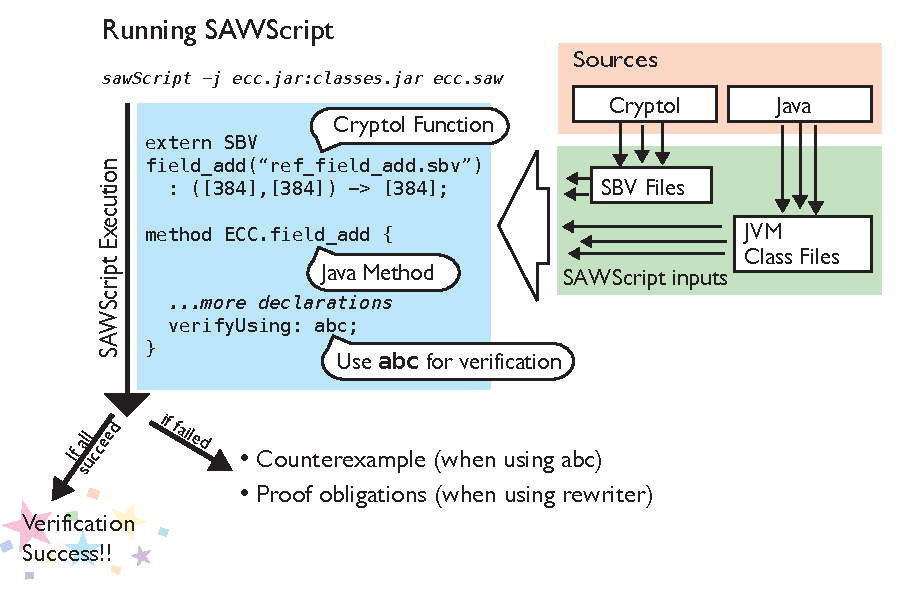
\includegraphics{figures/sawScriptExecution.pdf}
  \caption{\label{fig:sawScriptExecution} \sawScript verification workflow}
\end{center}
\end{figure}

Once the SBV files are obtained from Cryptol, we simply import them in \sawScript, using the {\tt extern SBV} command. As an example, we will
use an implementation of the field addition operation over the prime field underlying the P384 curve, coded in a Cryptol function with the following signature:
\begin{Verbatim}
   ref_p384_add : ([384],[384]) -> [384];
\end{Verbatim}
We will not need to know how {\tt ref\_p384\_add} itself is coded in Cryptol, as \sawScript will simply be using the SBV file corresponding to it.
We will assume that the SBV file is already generated and stored in a file named {\tt "sbv/ref\_p384\_add.sbv"}. We simply import
this file into \sawScript as follows:

\begin{code}
  extern SBV cry_fadd("sbv/ref_p384_add.sbv") : ([384],[384]) -> [384];
\end{code}

The above declaration tells \sawScript to load the SBV file and admit it as a function with the given type. (The type
annotation is mandatory. \sawScript will make sure that the declared type does indeed match what the SBV file defines.)

Once this declaration is given, we can refer to {\tt cry\_fadd} in our \sawScript proof as if it was one of the primitive functions
supported by \sawScript itself.

\subsection{Field addition}\label{sec:fieldadd}
Let us now turn to the Java implementation of {\tt field\_add}, which we will assume to have
been defined in the class {\tt com.galois.ecc.P384ECC64}, implementing
field addition for the prime field underlying the P384 curve~\cite[Section 2.8.1]{sec2}:
\begin{Verbatim}
  public void field_add(int[] z, int[] x, int[] y) {
      if (add(z, x, y) != 0 || leq(field_prime, z)) decFieldPrime(z);
  }
\end{Verbatim}
Note that we are {\em not} showing the definitions of {\tt add}, {\tt leq} or {\tt decFieldPrime}
functions here for brevity, as our specification will not need their details. The crucial thing to note is
that {\tt field\_add} is not a pure function: It will add the field elements represented by {\tt x} and {\tt y},
and store the result in {\tt z}, destructively updating its first argument. Hence, our \sawScript specification
will have to account for this state change.

The constant {\tt field\_prime} refers to the prime of the field underlying
P384. This constant is represented in the Java version using an int array with 12 elements. We will represent the field prime
in \sawScript, as given in the SEC documentation~\cite[Section 2.8.1]{sec2}:

\begin{code}
  let field_prime = <| 2^384 - 2^128 - 2^96 + 2^32 - 1 |> : [384];
\end{code}
Note the use of the polynomial notation as an aid in getting the specification looking as close as possible to the published
documentation.

Here is the \sawScript method specification for {\tt field\_add}:
\begin{code}[numbers=left]
  method com.galois.ecc.P384ECC64.field_add {
    var args[0], args[1], args[2] :: int[12];
    var this.field_prime :: int[12];
  
    mayAlias { args[0], args[1], args[2] };
  
    assert valueOf(this.field_prime) := split(field_prime) : [12][32];
  
    ensure valueOf(args[0]) := 
        split(cry_fadd( join(valueOf(args[1]))
                      , join(valueOf(args[2])))) : [12][32];
  
    verify abc;
  };
\end{code}
Let us go over this spec line by line, explaining how we constructed it:

\paragraph{Lines 1,2} As before, we indicate for which Java method the specification is written for, along with the types of the
arguments to the method. Again, the Java method takes arbitrary length integer arrays as arguments, but the use case
is for 384-bit numbers, which require an array of 12 32-bit Java {\tt int}s. Thus we fix the types at {\tt int[12]}.

\paragraph{Line 4} Whenever we have a Java method that takes multiple arguments as references, we have to be
concerned about aliasing. That is, whether the method arguments {\tt x}, {\tt y}, and {\tt z} might actually refer
to the same array. This is very important since {\tt field\_add} modifies {\tt z}, and it might have some
assumptions regarding whether {\tt z} might alias {\tt x}, {\tt y}, or both. Unfortunately, Java does not let programmers
to indicate aliasing explicitly, but our proof has to account for all possibilities.
By default, \sawScript assumes that reference arguments do {\em not} alias each other.
If this is not the case, then the user needs to tell \sawScript explicitly which arguments might alias each other. We do
this with a {\tt mayAlias} declaration, as illustrated in line 4. As the name {\tt mayAlias}
suggests, aliasing is {\em not} required: It just tells \sawScript to make sure the proof holds even if these arguments
can alias each other. (Naturally, adding aliasing constraints will make proofs more complicated to finish, but the specification complexity
will be hidden from the user.) In this case, we are telling
\sawScript that any two, or all three arguments to {\tt field\_add} might alias each other, i.e., refer to the same array.

\paragraph{Line 6} Remember that the Java method referred to the array {\tt field\_prime}, which happens to be a {\tt protected final}
field in {\tt com.galois.ecc.P384ECC64}. In line 6, we are telling \sawScript that the constant {\tt field\_prime}
we have defined above using the polynomial notation, and the Java value {\tt this.field\_prime} are indeed equivalent.
(Note that we have to use {\tt split} to turn our 384-bit field prime into a Java array, as Java represents {\tt field\_prime}
internally as an array.)

\paragraph{Lines 8-10} We now express the correctness condition for the {\tt field\_add} method. Since there is no return value for this
procedure, we cannot use a {\tt returns} statement. Instead, we express that the value of the first argument ({\tt args[0]}) will have 
changed in a certain way when the method completes execution. We do this with the {\tt ensures} statement on lines 8-10.
The specification simply says that if you take the values of {\tt args[1]} and
{\tt args[2]}, and then call the {\tt cry\_fadd} function we have imported from Cryptol,
then the result is what the value {\tt args[0]} will get assigned at the end of the method execution. That is, the
specification is simply:
\begin{Verbatim}
   // type incorrect, but illustrates the idea!
   ensures args[0] := cry_fadd(args[1], args[2]);
\end{Verbatim}
We simply have to insert calls to {\tt valueOf} to get values from Java into \sawScript, and split/join appropriately
to make sure the treatment of arrays and 384-bit words do match their intended usage. 

Note that the values of {\tt args[0]} and {\tt args[1]}
on the right hand side of the {\tt ensures} statement will refer to the initial values of the arguments when the method starts executing,
i.e., any changes to them due to aliasing will be properly accounted for in the proof.

\paragraph{Line 12} Finally, we give a hint to \sawScript to use bit-blasting and in particular the ABC tool to complete the proof. 

\paragraph{Note} To give a sense of the performance of \sawScript, the above proof completes in about 45 seconds on a decent commodity laptop.

\subsection{Field subtraction}
Similar to field addition, the correctness proof of field subtraction proceeds in a similar fashion:

\begin{code}
  extern SBV cry_fsub("sbv/ref_p384_sub.sbv") : ([384],[384]) -> [384];

  method com.galois.ecc.P384ECC64.field_sub {
    var args[0], args[1], args[2] :: int[12];
    var this.field_prime :: int[12];
    mayAlias { args[0], args[1], args[2] };
    assert valueOf(this.field_prime) := split(field_prime) : [12][32];
    ensure valueOf(args[0]) :=
         split(cry_fsub( join(valueOf(args[1]))
                       , join(valueOf(args[2])))) : [12][32];
    verify abc;
  };
\end{code}

(This particular method specification will come in handy when we attempt to prove the double decrement operation correct in Section~\ref{sec:doubledec}.)

Again, the proof for {\tt field\_sub} takes around 2 minutes to complete on a commodity laptop.

\subsection{Using assumptions}

The {\tt assume} directive tells \sawScript that a particular boolean expression can be assumed to hold when a proof is being attempted. This directive is
useful for stating invariants on the data. For instance, we can state:
\begin{Verbatim}
   assume is_field(join(valueOf(args[0]))); 
\end{Verbatim}
to state that the Java value of {\tt args[0]} satisfies the predicate {\tt is\_field}, which we might have
imported from an SBV file earlier:
\begin{Verbatim}
   extern SBV is_field("sbv/ref_p384_is_val.sbv") : [384] -> Bit;
\end{Verbatim}
When \sawScript sees this {\tt assume} directive, it will use it as a hypothesis during the proof, indicating that the method expects its inputs to
satisfy certain conditions. Note that the proof may not go through without this {\tt assume} statement, if the method does not guarantee to work
correctly when its inputs do not have the property indicated.

On the flip side of the coin,
any other method that uses a method with {\tt assume} directives will have to make sure that the required conditions do indeed hold when the call is made.
\sawScript will automatically track such dependencies and discharge them as appropriate, or the proof will fail with a bug identified.

\subsection{Indicating ``don't care'' conditions}

When \sawScript attempts a proof, it will make sure that {\em all} the changes made by the method are captured in {\tt ensures} statements. \sawScript
will not allow a proof to complete unless all of its side effects are properly accounted for.

It is, however, quite possible that a method
might be making some internal state changes that we really do not care about, as far as the verification tasks are concerned. For instance,
it is unlikely that we want to explicitly track changes to private class fields that are used for temporary storage purposes.
In such cases, we can use the {\tt arbitrary} directive to tell \sawScript to ignore any changes made to such references. For instance, the directive:
\begin{Verbatim}
  arbitrary: this.tmpBuffer;
\end{Verbatim}
tells \sawScript that the method changes the value of the class field {\tt tmpBuffer} during
its execution, but we do not care about such changes. If we omit this directive,
\sawScript will make sure that the field {\tt tmpBuffer} does {\em not} change during the execution of the method,
indicating a much stronger requirement.

\section{Using rules}\label{sec:rules}

The only verification technology we have so far employed in our \sawScript proofs is calling out to ABC, which essentially bit-blasts the problem
and applies SAT based reasoning. While this technique is suitable for a variety of verification tasks, it is not powerful enough to handle many
problems that crop up in cryptography due to large word sizes needed. For instance, a typical ECC algorithm will operate on 384-bit
words (or larger), and consequently will suffer from the classic state-explosion problem when bit-blasted. In particular, problems involving
multiplication are known to take time exponential to the word size of the variables involved, at least when using the current
SAT based technologies~\cite[Section 6.3.1]{DecisionProcedures2008}.

As an alternative proof technology, \sawScript comes with a rule-based rewrite engine to perform
traditional equational rewriting style proofs. This mode is selected using the directive:
\begin{Verbatim}
  verify rewrite;
\end{Verbatim}
Alternatively, the user can also tell \sawScript to first try rewriting, and then send the remaining unsolved goals to ABC, using the directive:
\begin{Verbatim}
  verify { rewrite; abc };
\end{Verbatim}
Note that the {\tt verifyUsing} directive is per method specification: Different specifications in the same \sawScript file can use different tactics.

In the remainder of this section we will illustrate how to use the rewriting engine to perform equivalence proofs of Java programs against their
Cryptol counterparts.

\subsection{Field double-decrement}\label{sec:doubledec}
As a simple example of how rewriting can significantly outperform a bit-blasting based proof, consider the operation of double decrementing a
field point that shows up often in ECC algorithms.
Given two field points $z$ and $x$, the double-decrement operation computes the value of $z - 2\times x$:
\begin{Verbatim}
  private void field_dbl_dec(int[] z, int[] x) {
    field_sub(z, z, x);
    field_sub(z, z, x);
  }
\end{Verbatim}
As usual, field-elements are represented as integer arrays, and we modify the first argument ($z$) directly to subtract the $x$ argument twice.
Note that the implementation is given as a procedure that modifies its first argument, as opposed to a pure function that returns a new result.
We can write the method specification for {\tt field\_dbl\_dec} as follows (note the use of the local {\tt let} bindings on lines 5 and 6 to improve readability):

\begin{Verbatim}[numbers=left]
  method com.galois.ecc.P384ECC64.field_dbl_dec {
    var args[0], args[1] : int[12];
    const valueOf(this.field_prime) := split(field_prime) : [12][32];
  
    let jarg0 = join(valueOf(args[0]));
    let jarg1 = join(valueOf(args[1]));
    ensures args[0] :=
         split(cry_fsub(cry_fsub(jarg0, jarg1), jarg1)) : [12][32];

    verifyUsing: abc;
  };
\end{Verbatim}

If you let \sawScript run this proof using bit-blasting you will
see that it indeed does finish the proof, in about 2 minutes of run time.

\subsection{Adding rules}
Let us try the double decrement proof again, this time using the rewriter. To do so, replace the
{\tt verifyUsing} command on line 10 as follows:

\begin{comment}
\begin{code}
  rule join_split: forAll {x:[384]}.  join(split(x) : [12][32]) -> x;

  rule eq_elim: forAll {x:a}. x == x -> true;

  method com.galois.ecc.P384ECC64.field_dbl_dec {
    var args[0], args[1] :: int[12];
    var this.field_prime :: int[12];
    assert valueOf(this.field_prime) := split(field_prime) : [12][32];
  
    let jarg0 = join(valueOf(args[0]));
    let jarg1 = join(valueOf(args[1]));
    ensure valueOf(args[0]) := split(cry_fsub(cry_fsub(jarg0, jarg1), jarg1)) : [12][32];
\end{code}
\end{comment}
\begin{code}
   verify rewrite;
\end{code}
\begin{comment}
\begin{code}
  };
\end{code}
\end{comment}
If you try now with \sawScript, you will get an immediate verification failure, indicating that the rewriter was not able to discharge
the verification condition. The reason for the failure is that the rewriter comes with no pre-installed rules on its own: \sawScript's
rewriter features a rewrite engine that makes no assumptions about the underlying domain, providing maximum flexibility to the user
for scripting the proof. This is the essence of the modular proof architecture featured by \sawScript, where users can guide the prover
to more and more efficient proofs by providing appropriate lemmas via rewrite rules.

Here is the error message from \sawScript:
\begin{Verbatim}
  The rewriter failed to reduce the verification condition generated
  from "args[0]" in the Java method
  com.galois.ecc.P384ECC64.field_dbl_dec to 'true'.
  The remaining goal is:
    (implies true
     (==
      (split
       (cry_fsub (join (split (cry_fsub{2} (join ?1) (join{1} ?0)))) n1))
      (split (cry_fsub n2 n1))))

  Please add new rewrite rules or modify existing ones to reduce the
  goal to true.
\end{Verbatim}

It will take a while for users to get familiar with \sawScript's internal term language, but the following is the essence of this message: When
the rewriter tried to show the equivalence, it was not able to {\em combine} the usages of calls to split and join.
In particular, we need to tell \sawScript that
splitting a large word into an array and joining it right back will produce precisely the same word. Thus, we add the following
rewrite rule:\footnote{Make sure to add the rule {\em before} the method specification, as otherwise it will not be taken into account during the proof.}
\begin{Verbatim}
  rule join_split: forAll {x:[384]}. join(split(x) : [12][32]) -> x;
\end{Verbatim}
What the above rule is stating that if we take a 384-bit value $x$, split it into an array of 12 elements each of which is 32 bits wide, and join it back
together, then we would get $x$ back. (See Section~\ref{sec:ruleanatomy} for more information on how rules are written.)

If you now try this proof, you will see that it fails again, with a slightly simpler unresolved term. Luckily, the rule we need in this case is trivial:
\begin{Verbatim}
  rule eq_elim: forAll {x:a}. x == x -> true;
\end{Verbatim}

After the addition of this rule (again before the method specification),
the proof will complete in less than a second! Compare this to the run-time of the pure bit-blasting based proof
which took about 2 minutes. The performance gains can be even more substantial for larger proofs. In fact, a rewriting
based proof might be the only means to complete a proof in practice, which would otherwise not be completed using reasonable amounts of time and/or memory with
existing SAT based technologies.

\subsection{How to determine the rules}
Perhaps the most difficult part of a rewrite based proof is to determine what rules to add to the system. As we have indicated before, \sawScript's rewriting
engine comes with
no hard-coded rules, to make sure we have a system that is as flexible as possible. However, it can be frustrating to determine what
rules a proof might need in order to discharge all verification conditions, especially for new users.
Aside from the need for getting used to the internal term language of \sawScript to understand
the unresolved goals, one needs to develop some intuitive understanding of how a rewriting based proof proceeds. We consider the tasks of determining and working
with the rules amongst the most important future development tasks for improving \sawScript's usability. In particular, we anticipate the need for being able
to group rules into rule sets that can be selectively applied at different times, along with facilities to automatically extract rules from
unresolved goals, all aimed at simplifying the proof construction process.

In the mean time, Galois intends to provide a set of rewrite rules that we have found to be useful in working with Java programs, especially those arising
in the domain of elliptic-curve cryptography. Galois will be making these rules available as a separate {\tt saw} file that users can simply import into their
own proof scripts and tweak as
needed. We believe that we can develop a robust set of rewrite rules that should simplify the proof construction tasks for the domain of cryptography
considerably.

\subsection{Anatomy of a rule}\label{sec:ruleanatomy}
To illustrate how rules are syntactically constructed, consider the following example stating that
append is associative:
\begin{Verbatim}
  rule appendAssoc:
        forAll {x:[a], y:[b], z:[c]}.  (x # y) # z -> x # (y # z);
\end{Verbatim}
Each rule is given a name, {\tt appendAssoc} above, which is used for diagnostic purposes. Following this, we list the
free variables mentioned in the rule body. For the {\tt appendAssoc} example, we have three variables, named {\tt x},
{\tt y}, and {\tt z}. Note that each parameter should be given an explicit type, although the type itself can be polymorphic.
For instance, the above rule states that {\tt x} is a word that has {\tt a} bits, {\tt y} is a word of size {\tt b} bits, etc.
Following this comes the method body, which consists of two expressions separated by {\tt ->}. The idea is that the left-hand-size
expression will be rewritten to the right-hand-side expression.
Note the directionality of the rule: While the underlying rule is actually an equation,
we syntactically write the rule in the form lhs {\tt ->} rhs, since the rewriter will never try to reduce the right-hand-side to
the left-hand-side.

This asymmetry is important for termination purposes, as we never want to create larger terms during a rewriting based proof. What "larger"
means in this context is not specified by \sawScript: In fact, \sawScript will not check that the given set of
rewrite rules will reduce the sizes of the
expressions as they are applied, so loops are certainly possible. For instance, a rule of the form:
\begin{Verbatim}
  rule badRule: forAll {x:[a], y:[a]}. x + y -> y + x;
\end{Verbatim}
would cause non-termination, as it will immediately create an expression that will trigger the rule again, ad infinitum. It is the
user's responsibility to make sure the rules are specified in a manner not to trigger such behavior.

The other important thing to note about rules is that their correctness is not checked by \sawScript. Once the rewrite rule is defined,
it is taken as is, regardless whether it actually represents a sound reduction. For instance, a rule of the form:
\begin{Verbatim}
  rule unsound: forAll {x:[a], y:[a]}. x + y -> y - x;
\end{Verbatim}
would render the system unsound. Note that this is not a fundamental restriction on the system, but rather a limitation of the current
implementation. In the future, we plan to incorporate means of verifying the correctness of rules themselves as well, at least for
certain monomorphic instances.

We conclude this section with a collection of example rules to give a flavor of what is expressible.

\paragraph{Array operations} The following rule captures how arrays operate:
\begin{code}
  rule getSet : forAll { a:[l]e, i:[idx], j:[idx], x:e }.
      aget(aset(a, i, x), j) -> if i == j then x else aget(a, j);
\end{code}
The rule states that if we update the element at index {\tt i} of an array {\tt a} with the value {\tt x}, and read that entry out,
we should get back {\tt x}. If we read some other index (i.e., when {\tt i} $\not=$ {\tt j}), then we should get back whatever
was stored in the array before the update took place.
Note how the rule is written polymorphically over arbitrary length arrays, indexes, and element types.

\paragraph{Rules about Cryptol functions} It is possible to state rules about functions that are
imported into \sawScript via Cryptol's SBV files. For instance, we can assert the following
rule about the {\tt cry\_fadd} function that we have imported from Cryptol in Section~\ref{sec:fieldadd}:

\begin{code}
  rule fieldAddAssoc : forAll {x:[384], y:[384], z:[384]}.
    cry_fadd (cry_fadd (x, y), z) -> cry_fadd (x, cry_fadd (y, z));
\end{code}

\paragraph{Simplifying {\tt if} expressions} As we have mentioned before, the rewriter comes with
no hard-coded rules, hence the following rules come in handy in simplifying {\tt if-then-else} expressions:

\begin{code}
  rule ifTrue : forAll {x:a, y:a}.     if true  then x else y -> x;
  rule ifFalse: forAll {x:a, y:a}.     if false then x else y -> y;
  rule ifNot  : forAll {c:Bit, d:Bit}. if c then d else true  -> not c || d;
  rule ifId   : forAll {c:Bit, d:Bit}. if c then true else d  -> c || d;
  rule ifEq   : forAll {c:Bit, x:a}.   if c then x else x     -> x;
\end{code}

\paragraph{If-then-else congruences} The following rules manipulate {\tt if-then-else} expressions,
pushing proof obligations to leafs:

\begin{code}
rule iteEq : forAll {b:Bit, x:a, y:a, z:a}.
    (if b then x else y) == z -> if b then (x == z) else (y == z);
rule iteSplit: forAll {b:Bit, x:[384], y:[384]}.
    split(if b then x else y) : [12][32] -> 
       if b then split(x) : [12][32] else split(y) : [12][32];
rule iteJoin: forAll {b:Bit, x:[12][32], y:[12][32]}.
    join(if b then x else y) -> if b then join(x) else join(y);
\end{code}

\paragraph{Boolean operations} Several rules relating how boolean connectives work:
\begin{code}
  rule and_true_elim1 : forAll {x:Bit}. true && x  -> x;
  rule and_true_elim2 : forAll {x:Bit}. x && true  -> x;
  rule and_false_elim1: forAll {x:Bit}. false && x -> false;
  rule and_false_elim2: forAll {x:Bit}. x && false -> false;
\end{code}

\paragraph{Record extraction} \sawScript supports structural records, similar to those found in Cryptol.
The following rules capture some field-selection properties related to records:

\begin{code}
  rule selX: forAll { xV:a, yV:b }. {x = xV; y = yV}.x -> xV;
  rule selY: forAll { xV:a, yV:b }. {x = xV; y = yV}.y -> yV;
\end{code}

We urge the reader to refer to the \sawScript distribution for a larger collection of rules that come in handy
for constructing proofs about ECC operations.

\subsection{Disabling/enabling rules}
As proof scripts get larger, users will inevitably find themselves needing tools for managing their \sawScript files.
In particular, the pair of directives:
\begin{Verbatim}
  disable r;
  enable r;
\end{Verbatim}
will tell the rewriting engine to stop/start using the rule named {\tt r}, respectively.
(When a rule is first defined, it is enabled by default.)

Similarly, we can also start/stop proofs as well. Recall that {\tt verifyUsing:} {\tt skip;}
tells \sawScript to skip the proof of a particular method. The directive
\begin{Verbatim}
  set verification off;
\end{Verbatim}
turns of proofs at that point, globally.
This is useful for skipping over a number of methods as far as proofs are concerned, so you can focus on later method specs in your proof
script. Analogously, you can use the directive
\begin{Verbatim}
  set verification on;
\end{Verbatim}
to re-enable verification.

\section{Summary}
In this document, we have introduced the \sawScript language, providing a means for end users to script functional equivalence proofs
using Galois's Java Verifier and Cryptol technologies. While we have designed \sawScript to be language agnostic, it is clearly
closely tied to Java and Cryptol for the time being. However, we do expect to be able to leverage this work and support other languages
in the future as well, such as LLVM or C. Furthermore, our current focus was on proving properties of programs that come up in the domain
of elliptic-curve cryptography. Research and development activities targeting extension to other domains of interest are clearly worth pursuing
as well.

While this document is intended to serve as an introductory material on basic \sawScript concepts, becoming a proficient \sawScript user will require
investment from end users, as with any other language or proof system. It is our hope that \sawScript will make formal proofs feasible for everyday
reasoning tasks, enabling the evaluators to achieve their goals in a more automated fashion. Any feedback, feature requests, or
comments on \sawScript is therefore most appreciated.
\newpage
\appendix
\section{\sawScript operators}
The following table lists all primitive \sawScript operators.

\begin{figure}[h]
\begin{center}
\begin{tabular}{c|c|l} \hline
Operator & Associativity & Notes \\ \hline\hline
{\tt not}, {\tt \url{~}}        & right & Boolean negation, and bitwise complement      \\ \hline
{\tt .}                         & left  & Record field selection                        \\ \hline
{\tt :}                         & left  & Type annotation                               \\ \hline
{\tt *}, {\tt /s}, {\tt \%s}    & left  & Multiplication, signed division and remainder \\ \hline
{\tt +}, {\tt -}                & left  & Addition and subtraction                      \\ \hline
{\tt <<}, {\tt >>s}, {\tt >>u}  & left  & Shift left, signed/unsigned shift right       \\ \hline
{\tt \&}                        & left  & Bit-wise and                                  \\ \hline
{\tt \Verb|^|}                  & left  & Bit-wise exclusive-or                         \\ \hline
{\tt \Verb+|+}                  & left  & Bit-wise or                                   \\ \hline
{\tt \#}                        & right & Concatenation                                 \\ \hline
{\tt ==}, {\tt !=}              & none  & Boolean equality, inequality                  \\ \hline
\parbox{3cm}{
\vspace*{0.5em}
{\tt >=s}, {\tt >=u}, {\tt >s}, {\tt >u}, {\tt <=s}, {\tt <=u}, {\tt <s}, {\tt <u}
\vspace*{0.5em}
}                               & none  & Signed/unsigned comparisons                   \\ \hline
{\tt \Verb+&&+}                 & left  & Boolean conjunction                           \\ \hline
{\tt \Verb+||+}                 & left  & Boolean disjunction                           \\ \hline
\end{tabular}
\end{center}
\caption{\sawScript operators: Higher precedence operators are listed first.
Operators in the same row are at the same precedence level, use parentheses to disambiguate if necessary.
Usual associativity rules do apply as well, as indicated in the table.}
\end{figure}

\paragraph{Modular arithmetic} All arithmetic ({\tt *}, {\tt +}, {\tt -}, {\tt /s}, {\tt \%s}, etc.) 
is performed modulo $2^s$, where $s$ is the bit-width of the operands. Both operands must have the same width.

\paragraph{Signed/unsigned operators} Some operators come in both signed and unsigned versions, such as comparisons ({\tt >u}, {\tt >s}, 
etc.), while some have only one version, such as shift-left ({\tt <<}) or multiplication ({\tt *}). \sawScript provides separate
operators when the signed versions are operationally different than unsigned ones, providing only
one operator if the signedness does not matter. To make the signedness absolutely
clear, all operators that have different semantics for signed/unsigned versions are tagged with the letters {\tt s} and {\tt u}, respectively.

\paragraph{Missing operators} Note that several operators are missing from this table, including unsigned division and remainder
({\tt /u}, {\tt \%u}), and left/right rotations. We plan to add these operators in future versions of \sawScript.

\newpage
\bibliography{sawScriptTutorial}
\addcontentsline{toc}{section}{References}
\bibliographystyle{abbrv}
\end{document}
